\chapter{Die Fourieranalyse -- Ordnung in komplexen Signalen}
\label{chap:fourieranalyse}
\index{Fourieranalyse}
\index{komplexe Signale}

\subsection{Einleitung: Verborgene Ordnung in komplexen Signalen}

\textbf{Leitfrage:}
Kann man komplexe Erscheinungen in einfache mathematische Bausteine zerlegen?

\medskip

Betrachtet man die Wellenform eines Musikstücks,
wirkt sie zunächst chaotisch und unübersichtlich.
Auch Sprache,
Meeresrauschen,
Licht oder technische Funksignale erscheinen auf den ersten Blick
wie komplizierte Muster ohne erkennbare Ordnung.

Dennoch zeigt die Mathematik:
Hinter vielen dieser scheinbar komplexen Signale
verbirgt sich eine erstaunlich einfache mathematische Struktur\index{Mathematische Struktur}.

Ein Musikton besteht beispielsweise nicht aus einer einzigen Schwingung,
sondern aus vielen überlagerten Frequenzen.
Die Fourieranalyse ermöglicht es,
diese einzelnen Bestandteile sichtbar zu machen.

Dadurch kann ein kompliziertes Signal
in einfache periodische Schwingungen zerlegt werden.
Die Mathematik erkennt also Ordnung dort,
wo zunächst nur Komplexität sichtbar ist.

\begin{DidacticBox}[Was ist ein komplexes Signal?]
	\small
	\label{box:fourier-komplexes-signal}
	Ein komplexes Signal besteht aus vielen überlagerten Schwingungen.
	
	Ein Klavierton enthält beispielsweise:
	
	\begin{itemize}
		\item einen Grundton,
		\item zahlreiche Obertöne,
		\item zeitliche Veränderungen,
		\item kleine Störungen und Nebengeräusche.
	\end{itemize}
	
	Trotzdem kann die Fourieranalyse diese Struktur mathematisch zerlegen
	und die einzelnen Frequenzanteile sichtbar machen.
\end{DidacticBox}

Die folgende Abbildung zeigt zunächst ein komplexes Signal,
wie es etwa bei einem Musikton auftreten kann.
Auf den ersten Blick wirkt die Kurve unregelmäßig.
Tatsächlich ist sie jedoch aus mehreren einfachen Schwingungen zusammengesetzt.

% ============================================================
% Bild 1: Komplexe Wellenform eines Tons
% ============================================================

\begin{figure}[h]
	\centering
	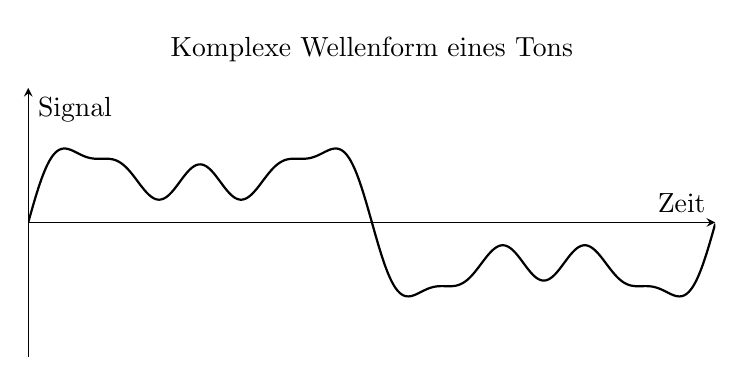
\begin{tikzpicture}
		\begin{axis}[
			width=0.85\textwidth,
			height=5cm,
			axis lines=middle,
			xlabel={Zeit},
			ylabel={Signal},
			xmin=0, xmax=6.28,
			ymin=-2.2, ymax=2.2,
			samples=500,
			domain=0:6.28,
			grid=both,
			xtick=\empty,
			ytick=\empty,
			title={Komplexe Wellenform eines Tons}
			]
			\addplot[thick]
			{sin(deg(x)) + 0.6*sin(deg(3*x)) + 0.35*sin(deg(5*x)) + 0.2*sin(deg(9*x))};
		\end{axis}
	\end{tikzpicture}
	\caption{Ein komplexes Signal wirkt zunächst unübersichtlich. Es kann jedoch aus mehreren einfachen Schwingungen zusammengesetzt sein.}
	\label{fig:komplexe-wellenform}
\end{figure}

Die Fourieranalyse zerlegt dieses Signal gedanklich
in einzelne harmonische Schwingungen.
Jede dieser Schwingungen besitzt eine eigene Frequenz und eine eigene Stärke.
Erst ihre Überlagerung ergibt die komplexe Wellenform.

% ============================================================
% Bild 2: Zerlegung in einzelne Sinuswellen
% ============================================================

\begin{figure}[h]
	\centering
	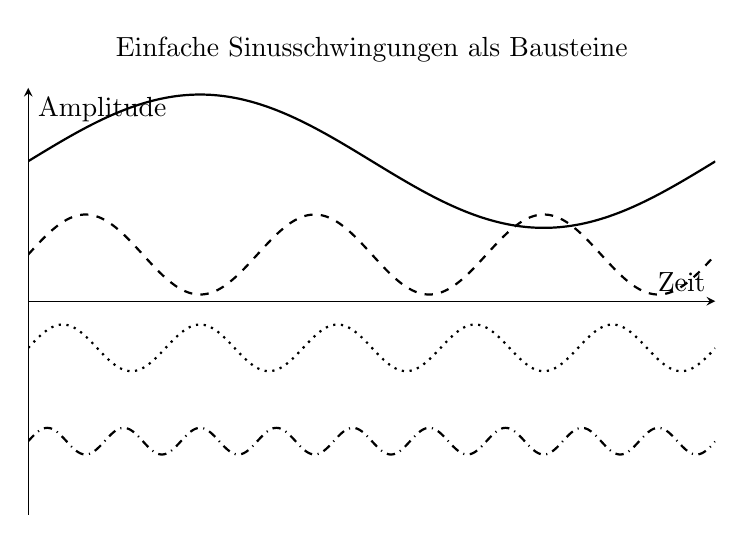
\begin{tikzpicture}
		\begin{axis}[
			width=0.85\textwidth,
			height=7cm,
			axis lines=middle,
			xlabel={Zeit},
			ylabel={Amplitude},
			xmin=0, xmax=6.28,
			ymin=-3.2, ymax=3.2,
			samples=400,
			domain=0:6.28,
			grid=both,
			xtick=\empty,
			ytick=\empty,
			title={Einfache Sinusschwingungen als Bausteine}
			]
			\addplot[thick] {sin(deg(x)) + 2.1};
			\addplot[dashed, thick] {0.6*sin(deg(3*x)) + 0.7};
			\addplot[dotted, thick] {0.35*sin(deg(5*x)) - 0.7};
			\addplot[dashdotted, thick] {0.2*sin(deg(9*x)) - 2.1};
			
			\node[anchor=west] at (axis cs:6.35,2.1) {\small Grundschwingung};
			\node[anchor=west] at (axis cs:6.35,0.7) {\small 3. Oberton};
			\node[anchor=west] at (axis cs:6.35,-0.7) {\small 5. Oberton};
			\node[anchor=west] at (axis cs:6.35,-2.1) {\small 9. Oberton};
		\end{axis}
	\end{tikzpicture}
	\caption{Die einzelnen Sinusschwingungen sind die mathematischen Bausteine des komplexen Signals. Zur besseren Sichtbarkeit sind sie hier vertikal versetzt dargestellt.}
	\label{fig:sinus-bausteine}
\end{figure}

Im Frequenzbereich wird schließlich sichtbar,
welche Frequenzen im Signal enthalten sind
und wie stark sie jeweils auftreten.
Die scheinbar komplizierte Wellenform erscheint dadurch plötzlich geordnet.

% ============================================================
% Bild 3: Frequenzspektrum
% ============================================================

\begin{figure}[h]
	\centering
	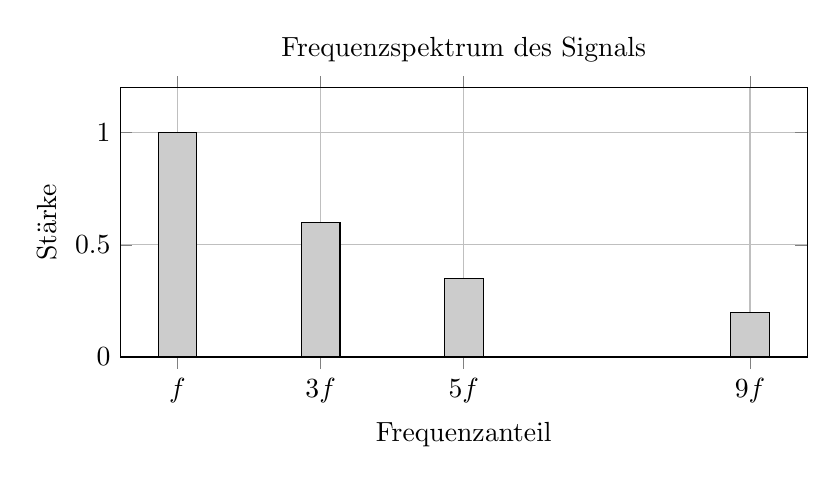
\begin{tikzpicture}
		\begin{axis}[
			width=0.85\textwidth,
			height=5cm,
			ybar,
			bar width=14pt,
			xlabel={Frequenzanteil},
			ylabel={Stärke},
			ymin=0, ymax=1.2,
			xtick={1,3,5,9},
			xticklabels={$f$,$3f$,$5f$,$9f$},
			grid=both,
			title={Frequenzspektrum des Signals}
			]
			\addplot[
			fill=gray!40,
			draw=black
			]
			coordinates {
				(1,1.0)
				(3,0.6)
				(5,0.35)
				(9,0.2)
			};
		\end{axis}
	\end{tikzpicture}
	\caption{Im Frequenzbereich erkennt man die verborgene Ordnung des Signals: wenige Frequenzanteile bestimmen seine Struktur.}
	\label{fig:frequenzspektrum}
\end{figure}

Die ursprüngliche komplizierte Wellenform erscheint im Frequenzbereich
plötzlich geordnet.
Man erkennt unmittelbar,
welche Frequenzen das Signal dominieren
und wie stark ihre jeweiligen Beiträge sind.

Die Fourieranalyse macht damit eine verborgene mathematische Struktur sichtbar,
die im ursprünglichen Signal kaum erkennbar war.
Sie zeigt beispielhaft,
wie Mathematik Ordnung sichtbar machen kann,
selbst wenn die Natur zunächst chaotisch erscheint.

% ============================================================
\subsection{Die Sprache der Schwingungen}

Schwingungen\index{Schwingung} gehören zu den grundlegendsten Erscheinungen der Natur.
Eine schwingende Gitarrensaite,
eine Wasserwelle
oder ein elektromagnetisches Signal
verändern sich periodisch mit der Zeit.

Besonders wichtig ist dabei die harmonische Schwingung\index{Harmonische Schwingung}.
Sie stellt die einfachste periodische Bewegung dar
und tritt näherungsweise überall dort auf,
wo ein System gleichmäßig um eine Ruhelage schwingt,
etwa bei einer Gitarrensaite,
einem Pendel
oder einer Stimmgabel.

Eine typische harmonische Schwingung lässt sich schreiben als

\[
y(t)=A\sin(2\pi f t+\varphi).
\]

Dabei bedeuten:

\begin{itemize}
	\item $A$ die Amplitude\index{Amplitude},
	\item $f$ die Frequenz\index{Frequenz},
	\item $\varphi$ die Phase\index{Phase},
	\item $t$ die Zeit.
\end{itemize}

Die Frequenz gibt an,
wie oft sich eine Schwingung pro Sekunde wiederholt.
Die Einheit der Frequenz ist das Hertz\index{Hertz} (Hz).

Die Amplitude beschreibt die Stärke der Schwingung.
Bei einem Ton entspricht sie beispielsweise der Lautstärke.

Die Phase gibt an,
an welcher Stelle innerhalb der periodischen Bewegung sich die Schwingung befindet.
Zwei Signale können dieselbe Frequenz besitzen,
aber zeitlich gegeneinander verschoben sein.

\begin{DidacticBox}[Was bedeutet „harmonische Schwingung“?]
	\small
	\label{box:fourier-harmonische-schwingung}
	Eine harmonische Schwingung ist die einfachste mögliche periodische Bewegung.
	
	Sie besitzt eine glatte,
	regelmäßige Form
	und wiederholt sich ständig.
	
	Sinus- und Kosinusfunktionen beschreiben solche Bewegungen besonders einfach.
	Darum bilden sie die mathematische Grundlage der Fourieranalyse.
\end{DidacticBox}

% ============================================================
% Bild 1: Niedrige und hohe Frequenz
% ============================================================

Die Frequenz bestimmt,
wie schnell sich eine Schwingung wiederholt.
Eine niedrige Frequenz besitzt nur wenige Schwingungen pro Zeitintervall,
eine hohe Frequenz dagegen viele.

\begin{figure}[h]
	\centering
	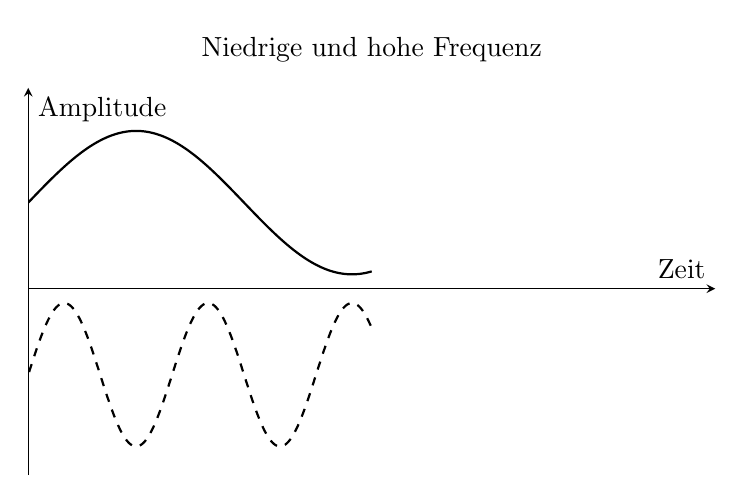
\begin{tikzpicture}
		\begin{axis}[
			width=0.85\textwidth,
			height=6.5cm,
			axis lines=middle,
			xlabel={Zeit},
			ylabel={Amplitude},
			xmin=0, xmax=10,
			ymin=-2.6, ymax=2.8,
			samples=500,
			grid=both,
			xtick=\empty,
			ytick=\empty,
			title={Niedrige und hohe Frequenz}
			]
			
			\addplot[thick]
			{sin(deg(x)) + 1.2};
			
			\addplot[dashed, thick]
			{sin(deg(3*x)) - 1.2};
			
			\node[anchor=west] at (axis cs:10.2,1.2)
			{\small niedrige Frequenz};
			
			\node[anchor=west] at (axis cs:10.2,-1.2)
			{\small hohe Frequenz};
			
		\end{axis}
	\end{tikzpicture}
	\caption{Die Frequenz beschreibt,
		wie schnell sich eine periodische Bewegung wiederholt.}
	\label{fig:frequenzvergleich}
\end{figure}

% ============================================================
% Bild 2: Unterschiedliche Amplituden
% ============================================================

Die Amplitude bestimmt die Stärke einer Schwingung.
Große Amplituden entsprechen stärkeren Ausschlägen,
kleine Amplituden schwächeren.

\begin{figure}[h]
	\centering
	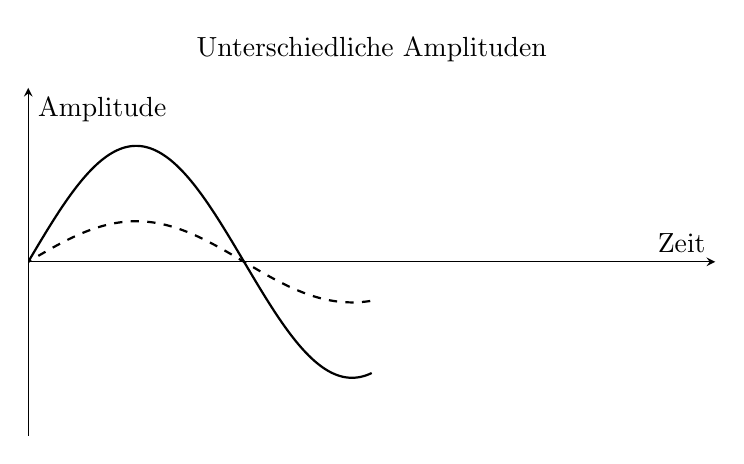
\begin{tikzpicture}
		\begin{axis}[
			width=0.85\textwidth,
			height=6cm,
			axis lines=middle,
			xlabel={Zeit},
			ylabel={Amplitude},
			xmin=0, xmax=10,
			ymin=-3, ymax=3,
			samples=500,
			grid=both,
			xtick=\empty,
			ytick=\empty,
			title={Unterschiedliche Amplituden}
			]
			
			\addplot[thick]
			{2*sin(deg(x))};
			
			\addplot[dashed, thick]
			{0.7*sin(deg(x))};
			
			\node[anchor=west] at (axis cs:10.2,2)
			{\small große Amplitude};
			
			\node[anchor=west] at (axis cs:10.2,0.7)
			{\small kleine Amplitude};
			
		\end{axis}
	\end{tikzpicture}
	\caption{Die Amplitude beschreibt die Stärke einer Schwingung.}
	\label{fig:amplitude}
\end{figure}

% ============================================================
% Bild 3: Phasenverschiebung
% ============================================================

Die Phase beschreibt die zeitliche Verschiebung einer Schwingung.
Zwei Signale können dieselbe Frequenz besitzen,
aber zeitlich gegeneinander verschoben sein.

\begin{figure}[h]
	\centering
	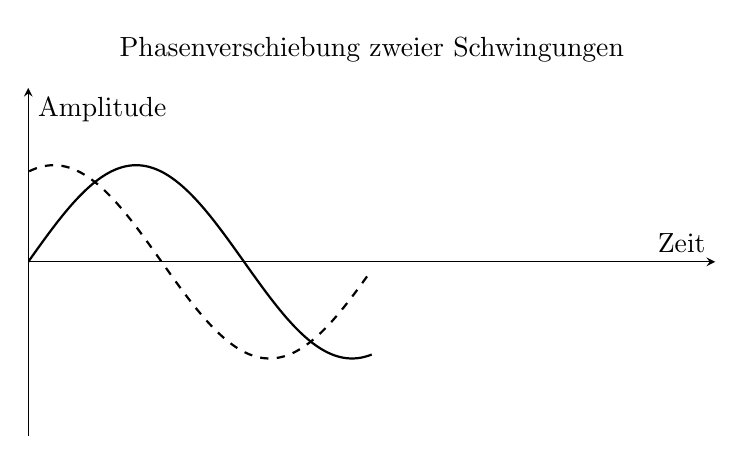
\begin{tikzpicture}
		\begin{axis}[
			width=0.85\textwidth,
			height=6cm,
			axis lines=middle,
			xlabel={Zeit},
			ylabel={Amplitude},
			xmin=0, xmax=10,
			ymin=-1.8, ymax=1.8,
			samples=500,
			grid=both,
			xtick=\empty,
			ytick=\empty,
			title={Phasenverschiebung zweier Schwingungen}
			]
			
			\addplot[thick]
			{sin(deg(x))};
			
			\addplot[dashed, thick]
			{sin(deg(x+1.2))};
			
			\node[anchor=west] at (axis cs:10.2,0.8)
			{\small ursprüngliche Schwingung};
			
			\node[anchor=west] at (axis cs:10.2,-0.8)
			{\small phasenverschobene Schwingung};
			
		\end{axis}
	\end{tikzpicture}
	\caption{Zwei Schwingungen mit gleicher Frequenz,
		aber unterschiedlicher Phase.}
	\label{fig:phase}
\end{figure}

\begin{MathBox}[Die Sinusfunktion als Grundbaustein]
	\small
	\label{box:fourier-sinus-grundbaustein}
	In der Fourieranalyse spielen Sinus- und Kosinusfunktionen
	eine besondere Rolle.
	
	Sie sind mathematisch einfach,
	periodisch
	und besitzen stabile Eigenschaften bei Ableitung und Integration.
	
	Dadurch eignen sie sich ideal als fundamentale Bausteine komplexer Signale.
\end{MathBox}

Sinus- und Kosinusfunktionen treten in der Natur besonders häufig auf,
weil viele physikalische Systeme bei kleinen Auslenkungen
näherungsweise harmonisch schwingen.
Darum spielen diese Funktionen in Physik und Technik eine zentrale Rolle.

Die Fourieranalyse untersucht schließlich nicht nur den zeitlichen Verlauf einer Schwingung,
sondern auch ihre Frequenzanteile.
Dadurch entsteht das sogenannte Frequenzspektrum\index{Frequenzspektrum}.

Man kann sich das Frequenzspektrum
wie eine Zerlegung eines Musikstücks in einzelne Töne vorstellen.
Anstatt das gesamte Signal gleichzeitig zu betrachten,
zeigt das Spektrum,
welche einzelnen Frequenzen darin verborgen sind.

Es zeigt also,
welche Frequenzen in einem Signal enthalten sind
und wie stark ihre jeweiligen Beiträge sind.

Damit wird sichtbar,
dass selbst komplizierte Signale oft aus wenigen grundlegenden Schwingungen aufgebaut sind.

% ============================================================
\subsection{Überlagerung: Wie komplexe Signale entstehen}

In der Realität treten reine Sinusschwingungen nur selten isoliert auf.
Meist überlagern sich viele verschiedene Frequenzen gleichzeitig.

Ein Musikton besteht beispielsweise nicht nur aus einem einzigen Grundton,
sondern zusätzlich aus zahlreichen Obertönen.
Diese bestimmen die charakteristische Klangfarbe eines Instruments.

Dadurch entsteht ein komplexes Signal,
das sich dennoch mathematisch als Summe einfacher Schwingungen beschreiben lässt.

Auch Sprache,
Meeresrauschen
oder technische Funksignale entstehen
durch die Überlagerung vieler unterschiedlicher Frequenzanteile.

\medskip

Die Idee der Überlagerung lässt sich an einem einfachen Beispiel verstehen.
Wirft man zwei Steine in ruhiges Wasser,
breiten sich zwei kreisförmige Wellen aus.
Treffen diese Wellen aufeinander,
so addieren sich ihre Ausschläge.

An manchen Stellen verstärken sich die Wellen gegenseitig,
an anderen schwächen sie sich ab.
Es entsteht ein vielschichtiges Muster,
obwohl jede einzelne Welle für sich genommen sehr einfach ist.

Ganz ähnlich entstehen auch komplexe Tonsignale.

\begin{DidacticBox}[Überlagerung von Wellen]
	\small
	\label{box:fourier-ueberlagerung-wellen}
	Wenn mehrere Schwingungen gleichzeitig auftreten,
	addieren sich ihre momentanen Auslenkungen.
	
	Diese Überlagerung nennt man Superposition\index{Superposition}.
	
	Komplexe Signale entstehen daher häufig
	durch die Kombination vieler einfacher Schwingungen.
\end{DidacticBox}

Bei einem Klavier erklingt beispielsweise nicht nur der Grundton einer Saite.
Zusätzlich entstehen zahlreiche Obertöne\index{Oberton} mit höheren Frequenzen.

Eine Flöte,
eine Geige
oder eine menschliche Stimme
besitzen jeweils unterschiedliche Mischungen solcher Frequenzanteile.
Dadurch klingt jedes Instrument charakteristisch,
selbst wenn derselbe Grundton gespielt wird.

Der Unterschied zwischen zwei Instrumenten,
die denselben Grundton spielen,
liegt also nicht im Grundton allein,
sondern in der Zusammensetzung der zusätzlichen Obertöne.
Die Fourieranalyse macht diese verborgene Struktur sichtbar.

Auch die menschliche Sprache entsteht durch komplexe Überlagerungen.
Beim Sprechen erzeugen Stimmbänder,
Mundraum
und Zunge ein sich ständig veränderndes Frequenzmuster.

Selbst scheinbar chaotische Geräusche wie Meeresrauschen oder Wind
bestehen letztlich aus einer Vielzahl überlagerter Frequenzen.

% ============================================================
% Bild 1: Überlagerung zweier Wellen
% ============================================================

Die folgende Abbildung zeigt,
wie aus zwei einfachen Schwingungen
durch Überlagerung ein komplexeres Signal entsteht.

\begin{figure}[h]
	\centering
	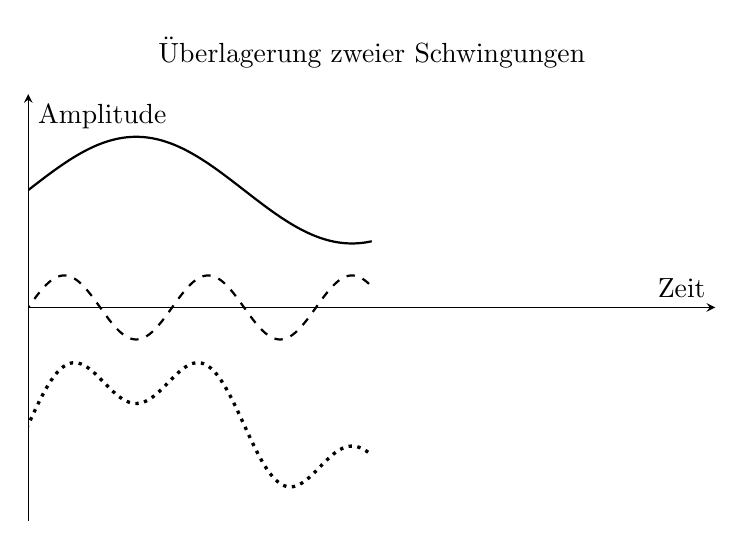
\begin{tikzpicture}
		\begin{axis}[
			width=0.85\textwidth,
			height=7cm,
			axis lines=middle,
			xlabel={Zeit},
			ylabel={Amplitude},
			xmin=0, xmax=10,
			ymin=-4, ymax=4,
			samples=500,
			grid=both,
			xtick=\empty,
			ytick=\empty,
			title={Überlagerung zweier Schwingungen}
			]
			
			% erste Schwingung
			\addplot[thick]
			{sin(deg(x)) + 2.2};
			
			% zweite Schwingung
			\addplot[dashed, thick]
			{0.6*sin(deg(3*x))};
			
			% Summe
			\addplot[dotted, very thick]
			{sin(deg(x)) + 0.6*sin(deg(3*x)) - 2.2};
			
			\node[anchor=west] at (axis cs:10.2,2.2)
			{\small Grundschwingung};
			
			\node[anchor=west] at (axis cs:10.2,0)
			{\small Oberton};
			
			\node[anchor=west] at (axis cs:10.2,-2.2)
			{\small Überlagerung};
			
		\end{axis}
	\end{tikzpicture}
	\caption{Zwei einfache Schwingungen ergeben durch Überlagerung ein komplexeres Signal.}
	\label{fig:ueberlagerung}
\end{figure}

Die untere Kurve entsteht dadurch,
dass sich die Ausschläge der beiden oberen Schwingungen
zu jedem Zeitpunkt addieren.

Bereiche mit gleichgerichteten Ausschlägen verstärken sich,
während sich entgegengesetzte Ausschläge teilweise abschwächen.

Schon aus wenigen einfachen Schwingungen
entsteht dadurch ein deutlich komplexerer Verlauf.

Die Mathematik zeigt damit,
dass komplexe Signale oft aus überraschend einfachen Bausteinen bestehen.

Genau diese Zerlegung komplexer Signale
in einfache Schwingungen
bildet die Grundlage der Fourieranalyse.

Die Fourieranalyse zeigt damit,
dass selbst scheinbar chaotische Strukturen
oft aus einfachen mathematischen Mustern aufgebaut sind.

% ============================================================
\subsection{Joseph Fourier und die große Idee}

Zu Beginn des 19.~Jahrhunderts beschäftigte sich der französische Mathematiker
Joseph Fourier\index{Fourier, Joseph} mit einem physikalischen Problem:
der Ausbreitung von Wärme\index{Wärmeleitung}.

Er untersuchte,
wie sich Temperatur in festen Körpern verändert,
wie Metallstäbe abkühlen
oder wie sich Wärme in der Erde ausbreitet.

Dabei stellte sich eine überraschende Frage:

\begin{NoteBox}[Ausgangspunkt der Fourieranalyse]
	\small
	\label{box:fourier-ausgangspunkt-waermeleitung}
	Wie kann man komplizierte Temperaturverläufe mathematisch beschreiben?
\end{NoteBox}

Fourier erkannte,
dass sich selbst sehr komplizierte Verteilungen
durch die Überlagerung einfacher periodischer Schwingungen darstellen lassen.

Diese Idee war revolutionär.

Bis dahin glaubten viele Mathematiker,
dass nur besonders glatte und regelmäßige Kurven
durch trigonometrische Funktionen beschrieben werden könnten.

Fourier behauptete jedoch:
Selbst eckige,
komplizierte
oder scheinbar unstetige Funktionen
lassen sich als Summe einfacher Sinus- und Kosinusfunktionen darstellen.

Heute erscheint diese Aussage selbstverständlich.
Damals war sie hoch umstritten.

Viele Zeitgenossen hielten Fouriers Ansatz zunächst für mathematisch fragwürdig.
Wie sollte eine eckige oder unstetige Kurve
aus glatten Sinusfunktionen zusammengesetzt sein?

Erst später erkannte man,
wie tiefgreifend Fouriers Idee tatsächlich war.

\begin{HistoryBox}[Joseph Fourier]
	\small
	\label{box:fourier-joseph-fourier}
	Joseph Fourier (1768--1830) entwickelte seine Theorie ursprünglich
	bei Untersuchungen zur Wärmeleitung.
	
	Seine Ideen gingen jedoch weit über dieses Gebiet hinaus
	und beeinflussten später Physik,
	Elektrotechnik,
	Signalverarbeitung,
	Astronomie
	und Quantenmechanik.
	
	Heute gehört die Fourier-Theorie
	zu den wichtigsten mathematischen Werkzeugen der modernen Wissenschaft.
\end{HistoryBox}

Die zentrale Aussage der Fourier-Theorie\index{Fourier-Theorie} lautet:
Jede periodische Funktion kann unter geeigneten Bedingungen als Überlagerung
von Sinus- und Kosinusfunktionen dargestellt werden.

Diese Aussage bedeutet,
dass selbst komplizierte Strukturen
oft aus einfachen periodischen Bausteinen zusammengesetzt sind.

Eine gezupfte Gitarrensaite,
ein Sprachsignal
oder ein digitales Tonsignal
erscheinen zunächst komplex.

Die Fourieranalyse zeigt jedoch,
dass sich hinter diesen Signalen
eine mathematische Ordnung verbirgt.

\begin{DidacticBox}[Warum Fouriers Idee revolutionär war]
	\small
	\label{box:fourier-revolutionaere-idee}
	Fourier zeigte,
	dass komplexe Kurven nicht zufällig oder chaotisch sein müssen.
	
	Selbst komplizierte Verläufe lassen sich
	auf einfache mathematische Schwingungen zurückführen.
	
	Damit entstand ein völlig neuer Blick
	auf Signale,
	Wellen
	und physikalische Prozesse.
\end{DidacticBox}

Ein besonders eindrucksvolles Beispiel ist das sogenannte Rechtecksignal\index{Rechtecksignal}.
Es besitzt abrupte Sprünge und scharfe Übergänge
und wirkt daher zunächst völlig unvereinbar
mit glatten Sinusfunktionen.

Die Fourier-Theorie zeigt jedoch,
dass sich selbst ein solches Signal
durch die Überlagerung harmonischer Schwingungen annähern lässt.

% ============================================================
% Bild: Rechtecksignal und Fourier-Näherung
% ============================================================

\begin{figure}[h]
	\centering
	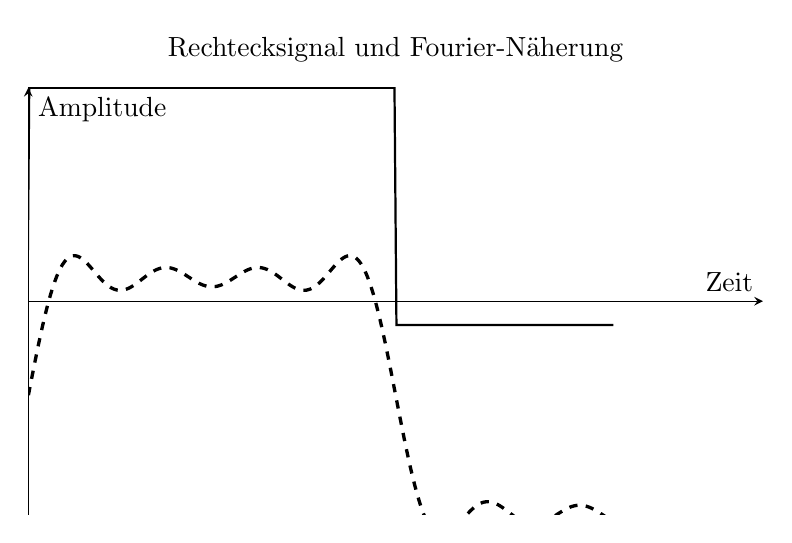
\begin{tikzpicture}
		\begin{axis}[
			width=0.9\textwidth,
			height=7cm,
			axis lines=middle,
			xlabel={Zeit},
			ylabel={Amplitude},
			xmin=0, xmax=6.28,
			ymin=-1.8, ymax=1.8,
			samples=600,
			grid=both,
			xtick=\empty,
			ytick=\empty,
			title={Rechtecksignal und Fourier-Näherung}
			]
			
			% Rechtecksignal
			\addplot[
			thick
			]
			{sign(sin(deg(x))) + 0.8};
			
			% Fourier-Näherung
			\addplot[
			dashed,
			very thick
			]
			{
				(4/pi) * (
				sin(deg(x))
				+ (1/3)*sin(deg(3*x))
				+ (1/5)*sin(deg(5*x))
				+ (1/7)*sin(deg(7*x))
				)
				- 0.8
			};
			
			\node[anchor=west] at (axis cs:6.4,0.8)
			{\small ideales Rechtecksignal};
			
			\node[anchor=west] at (axis cs:6.4,-0.8)
			{\small Fourier-Näherung};
			
		\end{axis}
	\end{tikzpicture}
	\caption{Selbst ein eckiges Rechtecksignal kann durch die Überlagerung mehrerer Sinusschwingungen angenähert werden.}
	\label{fig:rechteck-fourier}
\end{figure}

Die gestrichelte Kurve zeigt,
wie mehrere harmonische Schwingungen gemeinsam
ein Signal erzeugen,
das dem Rechtecksignal bereits erstaunlich ähnlich ist.

Damit wird sichtbar,
wie mächtig Fouriers Idee tatsächlich war:
Selbst scheinbar unregelmäßige oder abrupte Strukturen
können auf einfache mathematische Schwingungen zurückgeführt werden.

\begin{NoteBox}[Vertiefung: Rechtecksignal]
	\small
	\label{box:fourier-vertiefung-rechtecksignal}
	Das Rechtecksignal ist ein besonders anschauliches Beispiel für die Fourieranalyse:
	Eine sprunghafte, eckige Funktion lässt sich aus glatten Sinusschwingungen zusammensetzen.
	Die vollständige Herleitung der zugehörigen Fourier-Reihe steht in
	Anhang~A, Abschnitt~\ref{sec:anhang_fourieranalyse_rechtecksignal}.
\end{NoteBox}

Ursprünglich entstand die Fourieranalyse aus der Untersuchung der Wärmeleitung.
Später entwickelte sie sich jedoch zu einem universellen Werkzeug:
Sie wird heute in der Akustik, der Signalverarbeitung, der Quantenmechanik,
der Bildkompression und der digitalen Kommunikation verwendet.

% ============================================================
\subsection{Vom Zeitbereich zum Frequenzbereich}

Im Alltag betrachtet man Signale meist im Zeitbereich\index{Zeitbereich}.
Man untersucht,
wie sich ein Signal mit der Zeit verändert.

Ein Musiksignal erscheint dabei beispielsweise
als komplizierte Wellenform,
deren Verlauf sich ständig verändert.

Die Fourieranalyse ermöglicht jedoch eine völlig andere Sichtweise:
Statt nur den zeitlichen Verlauf zu betrachten,
analysiert man die enthaltenen Frequenzen.

Dadurch entsteht der sogenannte Frequenzbereich\index{Frequenzbereich}.

\medskip

Dieser Perspektivwechsel ist von zentraler Bedeutung.

Im Zeitbereich sieht man,
wie ein Signal verläuft.

Im Frequenzbereich erkennt man dagegen,
aus welchen Schwingungen das Signal zusammengesetzt ist.

Man kann sich dies ähnlich vorstellen
wie bei einem Musikstück:
Während man im Zeitbereich nur den gesamten Klang wahrnimmt,
zeigt der Frequenzbereich,
welche einzelnen Töne und Obertöne darin enthalten sind.

% ============================================================
% Bild: Zeitbereich und Frequenzbereich
% ============================================================

\begin{figure}[h]
	\centering
	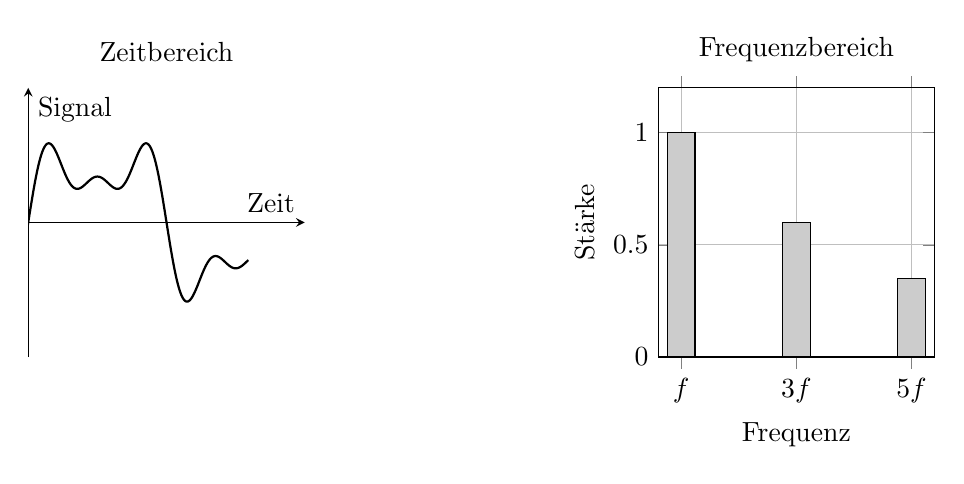
\begin{tikzpicture}
		
		% --------------------------------------------------------
		% Zeitbereich
		% --------------------------------------------------------
		
		\begin{axis}[
			width=0.42\textwidth,
			height=5cm,
			at={(0cm,0cm)},
			axis lines=middle,
			xlabel={Zeit},
			ylabel={Signal},
			xmin=0, xmax=6.28,
			ymin=-2.2, ymax=2.2,
			samples=500,
			grid=both,
			xtick=\empty,
			ytick=\empty,
			title={Zeitbereich}
			]
			
			\addplot[
			thick
			]
			{
				sin(deg(x))
				+ 0.6*sin(deg(3*x))
				+ 0.35*sin(deg(5*x))
			};
			
		\end{axis}
		
		\begin{axis}[
			width=0.42\textwidth,
			height=5cm,
			at={(8cm,0cm)},
			ybar,
			bar width=10pt,
			xlabel={Frequenz},
			ylabel={Stärke},
			ymin=0,
			ymax=1.2,
			xtick={1,3,5},
			xticklabels={$f$,$3f$,$5f$},
			grid=both,
			title={Frequenzbereich}
			]
			
			\addplot[
			fill=gray!40,
			draw=black
			]
			coordinates {
				(1,1.0)
				(3,0.6)
				(5,0.35)
			};
			
		\end{axis}
		
	\end{tikzpicture}
	\caption{
		Links sieht man das Signal im Zeitbereich.
		Rechts zeigt der Frequenzbereich,
		aus welchen Frequenzen das Signal zusammengesetzt ist.
	}
	\label{fig:zeit-frequenzbereich}
\end{figure}

Die Fourieranalyse zerlegt ein Signal also nicht nur mathematisch,
sondern verändert auch die Sichtweise auf das Problem.

Im Zeitbereich erscheint ein Signal oft kompliziert und unübersichtlich.
Im Frequenzbereich treten dagegen oft einfache und klar erkennbare Muster hervor.

Dadurch lassen sich verborgene Strukturen erkennen,
die im ursprünglichen Signal kaum sichtbar wären.

Die Fourieranalyse zeigt damit,
dass hinter scheinbar komplexen Signalen
oft eine verborgene mathematische Ordnung liegt.

\begin{NoteBox}[Zeitbereich und Frequenzbereich]
	\small
	\label{box:fourier-zeitbereich-frequenzbereich}
	Der Zeitbereich beschreibt,
	wie sich ein Signal im Verlauf der Zeit verändert.
	
	Der Frequenzbereich zeigt dagegen,
	welche Frequenzen im Signal enthalten sind
	und wie stark ihre jeweiligen Beiträge sind.
	
	Die Fourieranalyse verbindet beide Sichtweisen miteinander
	und macht dadurch verborgene Strukturen sichtbar.
\end{NoteBox}

\subsection{Anwendungen der Fourieranalyse}

\subsubsection*{Musik und Akustik}
\phantomsection

Die Fourier-Theorie spielt in der modernen Musiktechnik eine zentrale Rolle.

Elektronische Instrumente wie Synthesizer\index{Synthesizer} oder digitale Orgeln\index{Digitale Orgel}
erzeugen Klänge durch elektronische Schaltungen oder digitale Signalverarbeitung.

Dabei werden unterschiedliche periodische Wellenformen verwendet,
etwa Sinus-,
Rechteck-
oder Sägezahnschwingungen\index{Sägezahnschwingung}.

Durch die Kombination verschiedener Frequenzen
entstehen komplexe Klangfarben.

Die Fourier-Theorie beschreibt mathematisch,
wie sich solche komplexen Klänge
aus einfachen Schwingungen zusammensetzen lassen.

Dadurch wird verständlich,
warum unterschiedliche Instrumente trotz gleicher Tonhöhe
völlig verschieden klingen können.

\medskip

Auch die musikalische Notenschrift besitzt einen mathematischen Hintergrund.
Eine Note \index{Note}steht nicht nur für einen Ton,
sondern zugleich für eine bestimmte Tonhöhe und eine bestimmte Dauer.

Die Tonhöhe ist physikalisch mit der Frequenz einer Schwingung verbunden.
Je höher die Frequenz,
desto höher erscheint der Ton.
Eine Oktave \index{Oktave}entspricht dabei einer Verdopplung der Frequenz:
\[
f \longrightarrow 2f.
\]

Auch musikalische Intervalle beruhen auf Zahlenverhältnissen.
Eine Quinte l\index{Quinte}ässt sich näherungsweise durch das Frequenzverhältnis
\[
\frac{3}{2}
\]
beschreiben,
eine Quarte \index{Quarte}durch
\[
\frac{4}{3}.
\]

In der modernen gleichstufigen Stimmung wird die Oktave in zwölf gleiche Halbtonschritte \index{Halbtonschritte}unterteilt.
Der Frequenzfaktor zwischen zwei benachbarten Halbtönen \index{Halbtöne}beträgt daher
\[
2^{1/12}.
\]

Damit zeigt sich:
Musiknoten \index{Musiknote}sind nicht nur kulturelle Zeichen,
sondern verweisen auf eine mathematische Ordnung aus Frequenzen,
Zeitverhältnissen und Schwingungsstrukturen.

\begin{NoteBox}[Musiknoten als mathematische Ordnung]
	\small
	\label{box:Musiknoten}
	Eine Musiknote beschreibt nicht nur einen Klang,
	sondern auch mathematische Eigenschaften:
	Tonhöhe, Dauer, Rhythmus und Frequenzverhältnisse.
	
	Die Oktave entspricht einer Verdopplung der Frequenz,
	musikalische Intervalle beruhen auf Zahlenverhältnissen.
	Damit zeigt selbst die Notenschrift,
	dass Musik eine mathematische Struktur besitzt.
\end{NoteBox}

Synthesizer nutzen genau dieses Prinzip:
Sie kombinieren verschiedene Schwingungsformen und Frequenzen,
um künstliche Klänge zu erzeugen.
Die Fourier-Theorie liefert dazu die mathematische Beschreibung,
wie komplexe Klangstrukturen aus einfachen periodischen Schwingungen entstehen.

% ------------------------------------------------------------
\subsubsection*{Bild- und Signalverarbeitung}
\phantomsection

Die Fourieranalyse wird nicht nur bei Tönen und Schwingungen eingesetzt,
sondern auch bei Bildern\index{Bildverarbeitung}.

Das ist zunächst überraschend,
denn ein Bild scheint auf den ersten Blick nichts mit Schwingungen zu tun zu haben.
Mathematisch kann man jedoch auch ein Bild als Verteilung von Helligkeiten
und Farben auffassen.

Langsame Helligkeitsänderungen entsprechen niedrigen räumlichen Frequenzen\index{Räumliche Frequenz}.
Dazu gehören große Flächen,
weiche Übergänge
und grobe Formen.

Scharfe Kanten,
feine Details
oder Bildrauschen entsprechen dagegen hohen räumlichen Frequenzen.

\begin{DidacticBox}[Frequenzen in Bildern]
	\small
	\label{box:fourier-frequenzen-in-bildern}
	Bei Tönen beschreibt die Frequenz,
	wie schnell eine Schwingung zeitlich verläuft.
	
	Bei Bildern beschreibt eine räumliche Frequenz,
	wie schnell sich Helligkeit oder Farbe im Bild verändert.
	
	Große weiche Flächen besitzen niedrige Frequenzen,
	feine Details und Kanten hohe Frequenzen.
\end{DidacticBox}

Dieses Prinzip ist die Grundlage vieler Verfahren der Bildverarbeitung.

Bei der JPEG-Kompression\index{JPEG-Kompression} werden Bildinformationen so umgeordnet,
dass weniger wichtige Details stärker reduziert werden können.
Das menschliche Auge nimmt feine Änderungen in bestimmten Bildanteilen
oft weniger deutlich wahr.
Dadurch lässt sich die Datenmenge stark verringern,
ohne dass das Bild auf den ersten Blick wesentlich schlechter erscheint.

Auch bei der Rauschunterdrückung\index{Rauschunterdrückung} spielt die Frequenzanalyse eine wichtige Rolle.
Rauschen zeigt sich häufig als feines,
unregelmäßiges Muster.
Solche Anteile liegen oft im Bereich höherer Frequenzen
und können gezielt abgeschwächt werden.

Umgekehrt lassen sich Kanten und feine Strukturen hervorheben,
wenn hohe Frequenzanteile verstärkt werden.
Dadurch können Bilder geschärft
oder bestimmte Muster besser sichtbar gemacht werden.

An scharfen Kanten können dabei jedoch auch unerwünschte Effekte auftreten.
Besonders abrupte Helligkeitssprünge lassen sich durch Fourier-Näherungen
nicht vollkommen exakt darstellen.

Dabei entstehen kleine Über- oder Unterschwingungen,
die als Gibbs-Phänomen\index{Gibbs-Phänomen} bezeichnet werden.

Solche Effekte treten unter anderem
bei Bildkompression,
Signalfilterung
oder digitalen Audioverfahren auf.

\begin{DidacticBox}[Das Gibbs-Phänomen]
	\small
	\label{box:fourier-gibbs-phaenomen}
	Werden abrupte Sprünge oder scharfe Kanten
	durch Fourier-Reihen angenähert,
	entstehen in der Nähe dieser Übergänge
	charakteristische Überschwingungen.
	
	Dieses Verhalten nennt man Gibbs-Phänomen.
\end{DidacticBox}

Die folgende Abbildung zeigt das typische Überschwingen
einer Fourier-Näherung an einer sprunghaften Signaländerung.
Je mehr Fourier-Anteile verwendet werden,
desto glatter werden die Bereiche zwischen den Sprüngen.
Die Überschwingungen an den Sprungstellen bleiben jedoch charakteristisch erhalten.

% ============================================================
% Bild: Gibbs-Phänomen
% ============================================================
\begin{figure}[h]
	\centering
	\includegraphics[width=0.95\textwidth]{Bilder/gibbs-de.png}
	\caption{Das Gibbs-Phänomen: Eine Fourier-Näherung eines Rechtecksignals zeigt charakteristische Über- und Unterschwingungen an den Sprungstellen.}
	\label{fig:gibbs-bild}
\end{figure}

Auch wenn immer mehr Fourier-Anteile verwendet werden,
verschwindet das Überschwingen an der Sprungstelle nicht vollständig.

Das Gibbs-Phänomen zeigt damit,
dass die mathematische Approximation scharfer Übergänge
grundlegende Grenzen besitzt.

Ähnliche Überschwingeffekte treten auch in realen physikalischen Systemen auf.
Bei schnellen Schaltvorgängen in elektronischen Schaltungen,
etwa bei Transistoren oder digitalen Signalen,
zeigen sich häufig kurze Nachschwingungen oder Überspannungen.

Die Mathematik beschreibt damit nicht nur ein abstraktes Phänomen,
sondern erklärt auch reale Effekte moderner Technik.

Viele Verfahren der Bildverarbeitung beruhen darauf,
bestimmte Frequenzanteile zu verstärken,
abzuschwächen
oder zu entfernen.
So lassen sich Bilder komprimieren,
entrauschen,
schärfen
oder analysieren.

Die Fourieranalyse zeigt damit,
dass auch visuelle Information eine verborgene mathematische Struktur besitzt.
Ein Bild ist nicht nur eine Ansammlung von Pixeln,
sondern kann als Zusammenspiel räumlicher Muster verstanden werden.

% ------------------------------------------------------------
\subsubsection*{Medizinische Anwendungen}
\phantomsection

Auch in der modernen Medizin spielt die Fourieranalyse eine zentrale Rolle.

Viele medizinische Messverfahren liefern zunächst keine direkten Bilder,
sondern komplexe Signale,
die mathematisch ausgewertet werden müssen.

Erst durch die Analyse dieser Signale
lassen sich verborgene Strukturen des Körpers sichtbar machen.

\medskip

Ein besonders bekanntes Beispiel ist die Magnetresonanztomographie\index{Magnetresonanztomographie} (MRT\index{MRT}).

Dabei entstehen zunächst elektromagnetische Messsignale,
die Informationen über das Innere des Körpers enthalten.
Erst mithilfe mathematischer Verfahren,
unter anderem der Fourieranalyse,
können daraus detaillierte Schnittbilder rekonstruiert werden.

Die Mathematik wird damit zu einem Werkzeug,
das unsichtbare Strukturen des Körpers sichtbar macht.

\begin{PhysicsBox}[Mathematik macht den Körper sichtbar]
	\small
	\label{box:fourier-medizinische-bildgebung}
	Moderne medizinische Bildgebung basiert häufig nicht auf direkten Fotografien,
	sondern auf der mathematischen Analyse komplexer Signale.
	
	Die Fourieranalyse hilft dabei,
	aus diesen Messdaten Bilder und Strukturen des Körpers zu rekonstruieren.
\end{PhysicsBox}

Auch bei der Untersuchung von Gehirnaktivität spielt die Frequenzanalyse eine wichtige Rolle.

Beim Elektroenzephalogramm\index{Elektroenzephalogramm} (EEG\index{EEG})
werden elektrische Spannungen an der Kopfoberfläche gemessen.
Diese Signale bestehen aus unterschiedlichen Frequenzanteilen,
die mit verschiedenen Aktivitätszuständen des Gehirns verbunden sind.

So unterscheidet man beispielsweise:

\begin{itemize}
	\item Alpha-Wellen\index{Alpha-Wellen} (entspannter Wachzustand),
	\item Beta-Wellen\index{Beta-Wellen} (aktive Konzentration),
	\item Theta-Wellen\index{Theta-Wellen} (Schlaf- und Entspannungszustände).
\end{itemize}

Durch die Analyse dieser Frequenzmuster
lassen sich charakteristische Gehirnaktivitäten erkennen,
die im reinen Zeitverlauf oft nur schwer sichtbar wären.

Auch Ultraschallverfahren\index{Ultraschall} verwenden Prinzipien der Signal- und Frequenzanalyse.

Dabei werden reflektierte Schallwellen untersucht,
um Informationen über Gewebe,
Organe
oder Blutströmungen zu gewinnen.

Viele medizinische Verfahren messen zunächst nur Signale oder Wellen.
Erst die mathematische Analyse dieser Daten
macht daraus verständliche Bilder oder diagnostische Informationen.
Die Fourieranalyse verbindet damit Mathematik,
Physik
und moderne Medizin auf direkte Weise.

Die Fourieranalyse zeigt damit eindrucksvoll,
dass Mathematik nicht nur abstrakte Formeln beschreibt,
sondern hilft,
verborgene Strukturen des menschlichen Körpers sichtbar zu machen.

% ------------------------------------------------------------
\subsubsection*{Physik und Astronomie}
\phantomsection

In der Physik ermöglicht die Fourieranalyse die Untersuchung komplexer Wellenphänomene.

Viele physikalische Prozesse lassen sich als Überlagerung von Wellen beschreiben.
Die Fourier-Theorie hilft dabei,
diese Strukturen mathematisch zu analysieren
und verborgene Frequenzanteile sichtbar zu machen.

\medskip

Ein besonders wichtiges Beispiel ist die Spektralanalyse\index{Spektralanalyse} des Lichts.

Weißes Licht erscheint für das menschliche Auge zunächst einheitlich.
Tatsächlich besteht es jedoch aus vielen unterschiedlichen Wellenlängen beziehungsweise Frequenzen.

Durch ein Prisma oder ein Spektrometer
lässt sich das Licht in seine einzelnen Farbanteile zerlegen.

Bestimmte chemische Elemente absorbieren oder senden dabei ganz charakteristische Frequenzen aus.
Es entstehen sogenannte Spektrallinien\index{Spektrallinien}.

Dadurch können Astronomen bestimmen,
welche chemischen Elemente in Sternen oder Galaxien enthalten sind,
obwohl diese Objekte unvorstellbar weit entfernt sind.

\begin{PhysicsBox}[Spektrallinien als mathematische Signatur]
	\small
	\label{box:fourier-spektrallinien-signatur}
	Jedes chemische Element besitzt charakteristische Spektrallinien.
	
	Durch die Analyse der Frequenzen des ausgesandten oder absorbierten Lichts
	lässt sich bestimmen,
	welche Elemente in einem Stern enthalten sind.
	
	Die Mathematik wird damit zu einem Werkzeug,
	um Informationen über weit entfernte Objekte des Universums zu gewinnen.
\end{PhysicsBox}

Auch die Bewegung von Sternen und Galaxien lässt sich über Frequenzverschiebungen untersuchen.

Bewegt sich ein Stern von der Erde weg,
verschieben sich seine Spektrallinien zu längeren Wellenlängen.
Dieses Phänomen bezeichnet man als Rotverschiebung\index{Rotverschiebung}.

Auf ähnliche Weise können auch Geschwindigkeiten von Sternen,
Gaswolken
oder rotierenden Galaxien bestimmt werden.

\medskip

Die Fourieranalyse spielt außerdem in der modernen Quantenmechanik\index{Quantenmechanik} eine wichtige Rolle.

Teilchen werden dort häufig nicht nur als punktförmige Objekte beschrieben,
sondern auch durch Wellenfunktionen\index{Wellenfunktion}.

Ein lokalisiertes Teilchen kann mathematisch als Überlagerung vieler verschiedener Wellen dargestellt werden.
Solche Überlagerungen bezeichnet man als Wellenpakete\index{Wellenpaket}.

Die Fourier-Theorie verbindet dabei unterschiedliche Sichtweisen miteinander:
eine Beschreibung im Ortsraum\index{Ortsraum}
und eine Beschreibung im Impuls- beziehungsweise Frequenzraum\index{Impulsraum}.

\begin{DidacticBox}[Fourier-Theorie in der Quantenmechanik]
	\small
	\label{box:fourier-quantenmechanik}
	In der Quantenmechanik lassen sich viele Zustände
	als Überlagerung unterschiedlicher Wellen beschreiben.
	
	Die Fourier-Transformation\index{Fourier-Transformation} verbindet dabei
	den Ortsraum mit dem Impulsraum
	und gehört zu den grundlegenden mathematischen Werkzeugen der Theorie.
\end{DidacticBox}

Die Fourieranalyse zeigt damit eindrucksvoll,
dass dieselben mathematischen Prinzipien
sowohl bei Musik und Bildverarbeitung
als auch bei Sternenlicht und Quantenphysik auftreten.

Mathematik verbindet dadurch Bereiche,
die auf den ersten Blick völlig unterschiedlich erscheinen.

% ------------------------------------------------------------
\subsubsection*{Kommunikation und moderne Technik}
\phantomsection

Moderne Kommunikation\index{Datenübertragung} beruht darauf,
Informationen in Signale umzuwandeln.

Sprache,
Musik,
Bilder
oder digitale Daten
werden dabei als elektrische,
elektromagnetische
oder optische Signale übertragen.

Damit solche Signale zuverlässig übertragen werden können,
müssen sie analysiert,
gefiltert
und voneinander getrennt werden.

Genau hier spielt die Fourieranalyse eine zentrale Rolle.\index{Signalverarbeitung}

\medskip

Ein Mobilfunknetz\index{Mobilfunk} oder ein WLAN-System\index{WLAN} überträgt nicht einfach „Daten“ im abstrakten Sinn.
Die Information wird auf Trägerwellen gelegt,
die bestimmte Frequenzbereiche nutzen.

Verschiedene Nutzer,
Kanäle
oder Datenströme
können dadurch voneinander getrennt werden.

Moderne Kommunikationssysteme nutzen unterschiedliche Frequenzbereiche,
um Signale voneinander zu trennen.
Die Fourieranalyse hilft dabei,
diese Frequenzanteile zu erkennen,
zu filtern
und gezielt zu verarbeiten.

Auch bei der Glasfasertechnik\index{Glasfasertechnik} spielt dieses Prinzip eine wichtige Rolle.

Hier werden Informationen nicht über elektrische Ströme,
sondern über Lichtsignale übertragen.
Diese Lichtsignale können sehr schnell moduliert werden
und ermöglichen dadurch extrem hohe Datenraten.

Mehrere Datenkanäle können sogar über unterschiedliche Lichtwellenlängen
gleichzeitig durch dieselbe Glasfaser laufen.

Die Mathematik hilft dabei,
diese Signale sauber zu trennen
und Störungen möglichst gering zu halten.

% ============================================================
% Bild: Frequenzkanäle in der Kommunikation
% ============================================================

\begin{figure}[h]
	\centering
	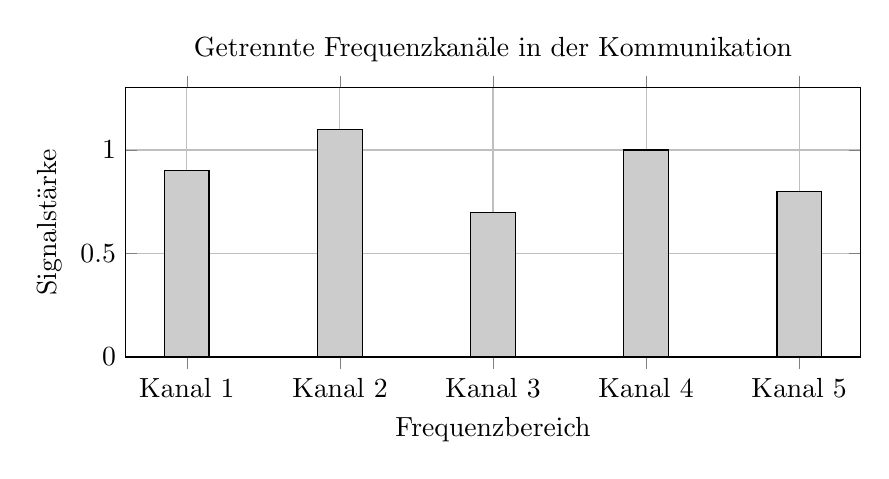
\begin{tikzpicture}
		\begin{axis}[
			width=0.9\textwidth,
			height=5cm,
			ybar,
			bar width=16pt,
			xlabel={Frequenzbereich},
			ylabel={Signalstärke},
			ymin=0,
			ymax=1.3,
			xtick={1,2,3,4,5},
			xticklabels={Kanal 1,Kanal 2,Kanal 3,Kanal 4,Kanal 5},
			grid=both,
			title={Getrennte Frequenzkanäle in der Kommunikation}
			]
			
			\addplot[
			fill=gray!40,
			draw=black
			]
			coordinates {
				(1,0.9)
				(2,1.1)
				(3,0.7)
				(4,1.0)
				(5,0.8)
			};
			
		\end{axis}
	\end{tikzpicture}
	\caption{
		Mehrere Signale können über unterschiedliche Frequenzbereiche
		getrennt übertragen und anschließend wieder herausgefiltert werden.
	}
	\label{fig:frequenzkanaele}
\end{figure}

Ein weiterer wichtiger Punkt ist die Trennung von Signal und Störung.

Reale Übertragungssysteme enthalten immer Rauschen,
Reflexionen
oder andere Störeinflüsse.
Durch Frequenzanalyse kann man erkennen,
welche Anteile zum gewünschten Signal gehören
und welche abgeschwächt oder herausgefiltert werden sollen.

Ohne solche mathematischen Verfahren wären moderne Datenübertragung,
Mobilfunk,
WLAN,
Satellitenkommunikation
und Glasfasertechnik kaum denkbar.

\begin{NoteBox}[Fourieranalyse als Grundlage der digitalen Welt]
	\small
	\label{box:fourier-digitale-welt}
	Die moderne Informationsgesellschaft beruht auf der Verarbeitung von Signalen.
	
	Ob WLAN,
	Mobilfunk,
	Satellitenverbindungen
	oder Glasfasertechnik:
	Überall müssen Frequenzen analysiert,
	getrennt,
	gefiltert
	und rekonstruiert werden.
	
	Die Fourieranalyse gehört damit zu den mathematischen Grundlagen
	der modernen Kommunikation.
\end{NoteBox}

Die Fourieranalyse zeigt hier besonders deutlich,
dass abstrakte Mathematik unmittelbare technische Bedeutung besitzt.

Sie macht es möglich,
Informationen zuverlässig zu übertragen,
Störungen zu reduzieren
und viele Datenströme gleichzeitig zu verarbeiten.

% ============================================================
\subsection{Die Fourieranalyse und die Struktur der Welt}

Die Fourieranalyse zeigt auf eindrucksvolle Weise,
dass hinter komplexen Erscheinungen oft einfache mathematische Muster verborgen liegen.

Was zunächst chaotisch,
unregelmäßig
oder unverständlich erscheint,
kann häufig durch die Überlagerung elementarer Schwingungen beschrieben werden.

Dies gilt für Musik,
Bilder,
elektrische Signale,
medizinische Messdaten,
Lichtspektren
und sogar für Wellenfunktionen der Quantenmechanik.

Überall taucht dieselbe mathematische Idee auf:
Komplexität entsteht aus der Kombination einfacher Strukturen.

Damit liefert die Fourieranalyse ein besonders starkes Beispiel
für die zentrale Leitidee dieses Buches:

\begin{NoteBox}[Mathematische Ordnung hinter komplexen Phänomenen]
	\small
	\label{box:fourier-mathematische-ordnung}
	Die Welt erscheint oft kompliziert und chaotisch.
	
	Doch hinter vielen Phänomenen verbirgt sich
	eine tiefe mathematische Struktur.
	
	Die Fourieranalyse zeigt,
	dass selbst komplexe Signale
	auf einfache Schwingungen zurückgeführt werden können.
\end{NoteBox}

Die Mathematik dient dabei nicht nur als Rechenwerkzeug,
sondern als Sprache,
mit der sich verborgene Ordnung sichtbar machen lässt.

Die Fourier-Theorie erzeugt diese Ordnung nicht --
sie entdeckt sie.

Gerade darin zeigt sich,
wie eng Mathematik und Realität miteinander verbunden sind.

Die Fourieranalyse macht sichtbar,
dass die Natur nicht aus isolierten Einzelphänomenen besteht,
sondern aus überlagerten Strukturen,
die mathematisch beschrieben werden können.

Damit wird die Mathematik zu einem Schlüssel,
mit dem sich die verborgene Struktur der Welt entschlüsseln lässt.
